\documentclass[12pt, a4papre]{article}
\usepackage[catalan]{babel}
\usepackage[unicode]{hyperref}
\usepackage{amsmath}
\usepackage{amssymb}
\usepackage{amsthm}
\usepackage{xifthen}
\usepackage{siunitx}
\usepackage{xcolor}
\usepackage{float}
\usepackage{listings}
\usepackage{setspace}
\usepackage{graphicx}
\usepackage{tikz,lipsum,lmodern}
\usepackage[most]{tcolorbox}
\usepackage{circuitikz}
\usepackage{indentfirst}
\usepackage{verbatimbox}
\definecolor{mygreen}{RGB}{28,172,0} % color values Red, Green, Blue
\definecolor{mylilas}{RGB}{170,55,241}
\usepackage{listings}
\lstdefinelanguage{vhdl}{
   morekeywords={
     library,use,all,entity,is,port,in,out,end,architecture,of,
     begin,and
   },
   morecomment=[l]--
}
\usepackage{xcolor}
\colorlet{keyword}{blue!100!black!80}
\colorlet{comment}{green!50!black!90}
\lstdefinestyle{vhdl}{
   language     = VHDL,
   basicstyle   = \ttfamily,
   keywordstyle = \color{keyword}\bfseries,
   commentstyle = \color{comment}
}

\graphicspath{ {./Imatges/} }


\newcommand{\norm}[1]{\lvert #1 \rvert}

\hypersetup{
    colorlinks = true,
    linkcolor = blue
}

\author{Daniel Vilardell\\
	   Igor Yuziv}
\title{Memoria Practica 2}
\date{}

\begin{document}
	\maketitle
	\newpage
	
	\textbf{\large{Conversor binari a BCD de 8 bits}}
	
	Aquest component el farem amb vhdl i te l'objectiu de convertir la sortida del multiplicador de 8 bits a bcd per tal de mostrar a la placa. Te la seguent forma
	\begin{lstlisting}[style=vhdl, frame=single, basicstyle=\tiny]
LIBRARY ieee; USE ieee.std_logic_1164.ALL;  

ENTITY BIN_BCD_8B IS PORT (   
	BIN : IN STD_LOGIC_VECTOR(7 downto 0);   
	BCD : OUT STD_LOGIC_VECTOR(7 downto 0)); 
END BIN_BCD_8B;  

ARCHITECTURE taula_veritat OF BIN_BCD_8B IS   
	BEGIN 
	with BIN SELECT BCD <=     	
		"10011001" WHEN "00111000",  -- 81     
		"01110010" WHEN "01001000",  -- 72      
		"01100100" WHEN "01000000",  -- 64     
		"01010110" WHEN "00111000",  -- 56     
		"01010100" WHEN "00111000",  -- 54        
		"01001001" WHEN "00110001",  -- 49     
		"01001000" WHEN "00110000",  -- 48     
		"01000101" WHEN "00101101",  -- 45     
		"01000010" WHEN "00101010",  -- 42     
		"01000000" WHEN "00101000",  -- 40     
		"00110110" WHEN "00100100",  -- 36     
		"00110101" WHEN "00100011",  -- 35     
		"00110010" WHEN "00100000",  -- 32     
		"00110000" WHEN "00011110",  -- 30     
		"00101000" WHEN "00011100",  -- 28     
		"00100110" WHEN "00011011",  -- 27     
		"00100101" WHEN "00011001",  -- 25     
		"00100100" WHEN "00011000",  -- 24     
		"00100001" WHEN "00010101",  -- 21     
		"00100000" WHEN "00010100",  -- 20     
		"00011000" WHEN "00010010",  -- 18     
		"00010110" WHEN "00010000",  -- 16     
		"00010101" WHEN "00001111",  -- 15     
		"00010100" WHEN "00001110",  -- 14     
		"00010010" WHEN "00001100",  -- 12     
		"00010000" WHEN "00001010",  -- 10     
		"00001001" WHEN "00001001",  -- 9     
		"00001000" WHEN "00001000",  -- 8     
		"00000111" WHEN "00000111",  -- 7     
		"00000110" WHEN "00000110",  -- 6     
		"00000101" WHEN "00000101",  -- 5     
		"00000100" WHEN "00000100",  -- 4    
		"00000011" WHEN "00000011",  -- 3     
		"00000010" WHEN "00000010",  -- 2     
		"00000001" WHEN "00000001",  -- 1     
		"00000000" WHEN "00000000",  -- 0     
		"--------" WHEN OTHERS;   
END taula_veritat;
\end{lstlisting}
	
	\textbf{\large{Conversor de binari de 4 bits a 8 bits}}
	
	Aquest component el conectarem abans de la entrada del multiplicador per a transformar la entrada de 4 bits a la que necessita el multiplicador que es de 8 bits. Aquest l'unic que farà es omplir de 0 les primeres 4 entrades.
	\begin{figure}[H]
		\begin{center}
		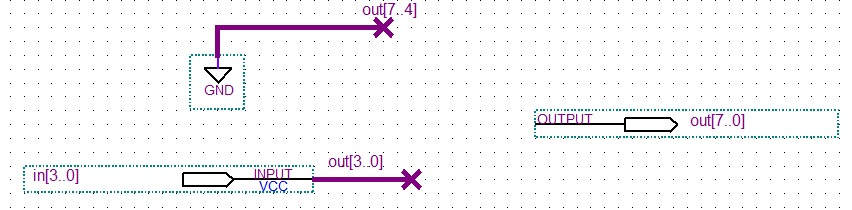
\includegraphics[width=130mm]{Bin_4_8.jpeg}
		\end{center}
	\end{figure}
	
	\textbf{\large{Multiplicador}}
	
	Aquest component t'he l'objectiu de multiplicar 2 nombres de 4 bits i treure la sortida en BCD de 4 bits, es a dir, 8 bits de sortida. Per a fer això usarem el component creat a la practica anterior que et multiplicava dos nombres de 8 bits. A la entrada hi posarem un conversor de 4 a 8 bits i a la sortida un conversor de binari de 8 bits a BCD que crearem amb vhdl.
	
	\begin{figure}[H]
		\begin{center}
		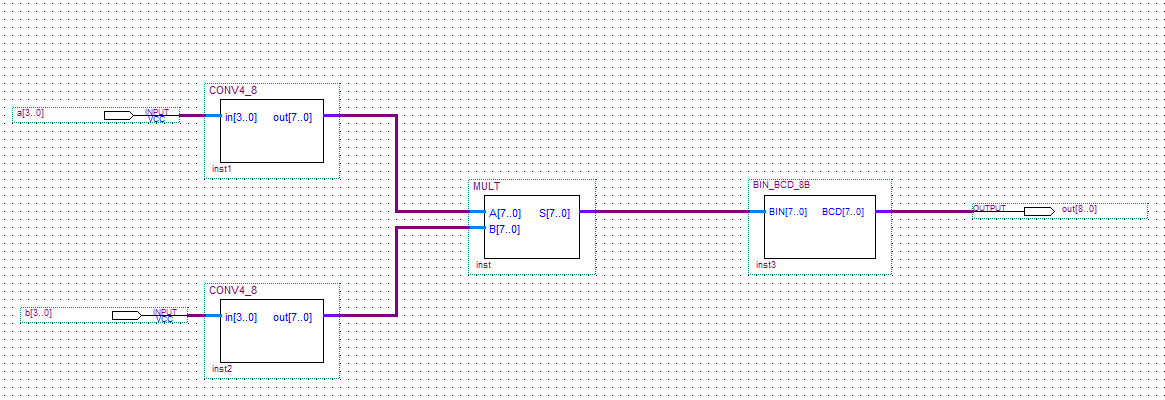
\includegraphics[width=130mm]{Mult_Bin_BCD.jpeg}
		\end{center}
	\end{figure}
	
	\textbf{\large{Bloc sel}}
	
	Aquest bloc te l'objectiu de retornar un bus de 7 bits amb el nombre $a$ si la entrada $show$ es 1, i 1111111 si la entrada $show$ es 0;
	\begin{figure}[H]
		\begin{center}
		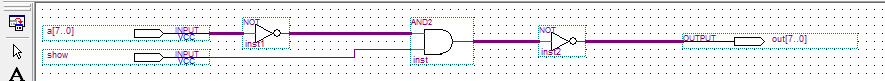
\includegraphics[width=130mm]{SEL.jpeg}
		\end{center}
	\end{figure}
	
	\begin{figure}[H]
		\begin{center}
		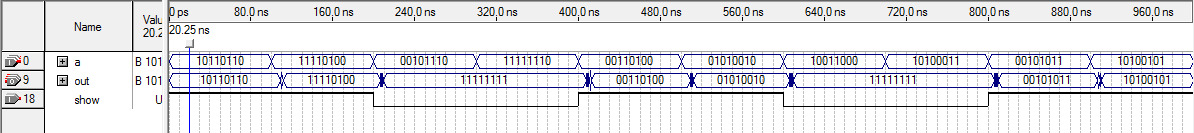
\includegraphics[width=130mm]{Simulacio_Sel.jpeg}
		\end{center}
	\end{figure}
		
\end{document}